\color{cyan} %color de texto con 70-80 % o más de avance
\section{Sensado remoto, plataformas (¿?) (Bloque 1)}
\subsection{Requerimientos y restricciones}
Para llevar adelante el relevamiento de las áreas forestales hay que tener en cuenta los requerimientos en el tiempo y en el equipamiento, así como las restricciones que imponen las regulaciones legales y condiciones geográficas y meteorológicas. Dependiendo de cuán grande sea el área a relevar, puede resultar más conveniente alguna de las plataformas de sensado remoto que otra. El criterio que debe ponderarse está basado en cálculos de tiempo, de costos operacionales y de disponibilidad. Para distintos escenarios, reservas grandes de miles de hectáreas de extensión o pequeñas reservas privadas de pocas decenas o centenas de hectáreas, los cálculos arrojarán resultados diferentes.
\subsubsection{Cálculo de factor de escala}
Los sensores remotos que serán tratados en el presente trabajo son del tipo pasivo, es decir, están compuestos por detectores que registran las ondas de luz solar reflejadas en el terreno. Particularmente nos interesan los que cubren el espectro visible. Básicamente constituyen una cámara fotográfica, que se compone de un arreglo de lentes y espejos que refractan y reflejan la luz, proyectándola sobre un sensor fotosensible, generalmente es un rectángulo conformado como un arreglo de detectores, cada uno de ellos representa a un pixel de la imagen. Según las características de estos sensores y la configuración de lentes, la distancia al objetivo, la resolución espacial queda determinada. 
Para poder comparar entre las diferentes opciones de plataformas para captura de imágenes aeroespaciales, es necesario conocer determinados parámetros de cada una. Un parámetro es el tiempo necesario para captura de imágenes de un determinado área. El costo asociado a la operación de captura de imágenes es otro parámetro a ser tenido en cuenta. Finalmente hay otros parámetros sobre los que las opciones pueden soportarse. Uno es el porcentaje de área útil sobre área total relevada. Otro parámetro es el espacio de almacenamiento requerido.
Si se comparan imágenes obtenidas por satélites contra aquellas obtenidas por aeronaves tripuladas o VANT, resulta evidente que aquellas cubren una extensión mayor, por lo que una sola captura puede exceder en mucho la zona de interés. En el caso de las imágenes aéreas es muy probable que sean necesarias varias imágenes para cubrir la zona de interés. Si se pretende construir un ortomosaico con esas imágenes, es necesario garantizar al momento de realizar las capturas un mínimo nivel de solapamiento entre capturas consecutivas (60\%) y entre aquellas que pertenecen a líneas de vuelo adyacentes (25\%). Los satélites son básicamente cámaras que orbitan alrededor del planeta que capturan imágenes de manera regular, continua, las cuales se  almacenan temporalmente en el satélite y son descargadas a estaciones de enlace para luego ser comercializadas. De modo que a requerimiento, las imágenes suelen estar disponibles. diferente es el caso de las imágenes aéreas, para las cuales se define un vuelo específico- Eso conlleva otros tiempos, ya que implica programar y preparar el vuelo, eventualmente trasladar la aeronave si es tripulada desde el aeródromo del cual despega y al cual regresa para aterrizar, y la duración misma del procedimiento de captura. Entre las variables que intervienen en la duración del vuelo en la fase de captura de imágenes se puede mencionar la de la extensión del área de interés, la velocidad de desplazamiento, la altura de vuelo. Esto también tendrá incidencia en la resolución espacial de las imágenes y en el espacio de almacenamiento requerido. Finalmente en el costo total del procedimiento, en el caso de aeronaves tripuladas incidirá el tiempo que lleve desde la puesta en marcha del motor hasta su apagado, ya que todo eso se contempla como hora de vuelo.
Los sensores, esto es, las cámaras que son llevadas como carga útil por las diferentes plataformas, están definidos por sus características. La distancia focal es un atributo de cada cámara. El factor de escala está dado por la altura de vuelo sobre el terreno, que puede variar incluso durante el vuelo, y por la distancia focal de la cámara, que es fija. 
\begin{figure}
    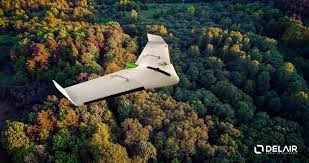
\includegraphics[width=\textwidth]{Imagenes/dron.jpg}
     \hfill
     \caption{Acá puede ir o no una imagen ilustrativa; revisar que esté referenciada correctamente}
    \label{dron}
\end{figure}
Para hallar el factor de escala $m_b$, relacionamos la altura de vuelo $H_g$ con la distancia focal
de la cámara $f$ mediante la ecuación \ref{escala} \cite{linder_digital_2016}:
 %%%%%%%%%%%%%%%%%%%%%%%%%%%%%%%%%%%%%% ECUACIÓN %%%%%%%%%%%%%%%%%%%%%%%%%%%%%%%%%%%%%%%%%%%%%%%%%%%%%%%%%
\\
\begin{equation}
	m_b=\frac{H_g}{f},\label{escala}
\end{equation}
\\
%%%%%%%%%%%%%%%%%%%%%%%%%%%%%%%%%%%%%%%%%%%%%%%%%%%%%%%%%%%%%%%%%%%%%%%%%%%%%%%%%%%%%%%%%%%%%%%%%%%%%%%%%
Para hallar cualquier distancia en la superficie real a partir de la fotografía, se aplica la relación de escala:
 %%%%%%%%%%%%%%%%%%%%%%%%%%%%%%%%%%%%%% ECUACIÓN %%%%%%%%%%%%%%%%%%%%%%%%%%%%%%%%%%%%%%%%%%%%%%%%%%%%%%%%%
\\
\begin{equation}
	S=\frac{S'H_g}{f},\label{escala1}
\end{equation}
\\
%%%%%%%%%%%%%%%%%%%%%%%%%%%%%%%%%%%%%%%%%%%%%%%%%%%%%%%%%%%%%%%%%%%%%%%%%%%%%%%%%%%%%%%%%%%%%%%%%%%%%%%%%
donde $S$ es la distancia en la superficie real, $S'$ es la distancia en la imagen.
En un relevamiento fotogramétrico, el solapamiento longitudinal suele ser de un promedio de 60\%, mientras que el solapamiento lateral suele ser de 25\% [4]. La distancia longitudinal $B$ entre dos fotografías consecutivas (línea de base) se halla en función al solapamiento longitudinal $p$, y se calcula según la ecuación (\ref{linea_de_base}).
 %%%%%%%%%%%%%%%%%%%%%%%%%%%%%%%%%%%%%% ECUACIÓN %%%%%%%%%%%%%%%%%%%%%%%%%%%%%%%%%%%%%%%%%%%%%%%%%%%%%%%%%
\\
\begin{equation}
	B=S(1-\frac{p}{100}),\label{linea_de_base}
\end{equation}
\\
%%%%%%%%%%%%%%%%%%%%%%%%%%%%%%%%%%%%%%%%%%%%%%%%%%%%%%%%%%%%%%%%%%%%%%%%%%%%%%%%%%%%%%%%%%%%%%%%%%%%%%%%%
La distancia $a$ entre dos líneas de sobrevuelo adyacentes se define por el solapamiento lateral $q$.
  %%%%%%%%%%%%%%%%%%%%%%%%%%%%%%%%%%%%%% ECUACIÓN %%%%%%%%%%%%%%%%%%%%%%%%%%%%%%%%%%%%%%%%%%%%%%%%%%%%%%%%%
\\
\begin{equation}
	a=S(1-\frac{q}{100}),\label{distancia_adyacente}
\end{equation}
\\
%%%%%%%%%%%%%%%%%%%%%%%%%%%%%%%%%%%%%%%%%%%%%%%%%%%%%%%%%%%%%%%%%%%%%%%%%%%%%%%%%%%%%%%%%%%%%%%%%%%%%%%%%
Cuando se trata de un vuelo para realizar fotografías aéreas, ya sea tripulado o no, partiendo de conocer el área de interés, sus dimensiones, es posible definir las trayectorias de vuelo. De esta forma el relevamiento fotográfico aéreo se asemeja a una especie de "barrido", con varias líneas adyacentes. A lo largo de una línea se capturan imágenes de modo que se superpongan como mínimo en un 80\% dos fotografías consecutivas. Al final de cada línea la aeronave ejecuta un giro de 180º respecto al eje nadir-cenit de modo que al finalizar el giro su proa apunte en dirección contraria a la que tenía antes de iniciar el giro. Así inicia el recorrido de una nueva línea de vuelo, la cual es paralela a la anterior, separada una distancia que garantice un solapamiento mínimo de 25\%de imágenes en líneas de vuelo adyacentes. A partir de todo ello puede establecerse la cuenta de imágenes totales que cubran toda el área, así como el tiempo necesario para llevarlo a cabo. De esto también se obtiene el espacio de almacenamiento en memoria requerido.
La cantidad de imágenes por línea de vuelo $I_lv$ se puede conocer dada la longitud de la línea de vuelo $L_v$ y la línea de base $B$, mediante la ecuación (\ref{cantidad_imagenes}):
  %%%%%%%%%%%%%%%%%%%%%%%%%%%%%%%%%%%%%% ECUACIÓN %%%%%%%%%%%%%%%%%%%%%%%%%%%%%%%%%%%%%%%%%%%%%%%%%%%%%%%%%
\\
\begin{equation}
	I_{lv}=\frac{L_v}{B},\label{cantidad_imagenes}
\end{equation}
\\
%%%%%%%%%%%%%%%%%%%%%%%%%%%%%%%%%%%%%%%%%%%%%%%%%%%%%%%%%%%%%%%%%%%%%%%%%%%%%%%%%%%%%%%%%%%%%%%%%%%%%%%%%
Multiplicando el resultado de la ecuación \ref{cantidad_imagenes} por la cantidad de líneas de vuelo $N_{lv}$ se obtiene la cantidad total de imágenes $I_t$ para toda el área relevada:
  %%%%%%%%%%%%%%%%%%%%%%%%%%%%%%%%%%%%%% ECUACIÓN %%%%%%%%%%%%%%%%%%%%%%%%%%%%%%%%%%%%%%%%%%%%%%%%%%%%%%%%%
\\
\begin{equation}
	I_t={I_{lv}}{N_{Lv}},\label{cantidad_total_imagenes}
\end{equation}
\\
%%%%%%%%%%%%%%%%%%%%%%%%%%%%%%%%%%%%%%%%%%%%%%%%%%%%%%%%%%%%%%%%%%%%%%%%%%%%%%%%%%%%%%%%%%%%%%%%%%%%%%%%%
El espacio de almacenamiento necesario de cada imagen $M_i$ está determinado por las características de los sensores, la cantidad de píxeles $Px$, cantidad de bandas espectrales $B_e$, la profundidad en bits de cada canal $Pb$:
  %%%%%%%%%%%%%%%%%%%%%%%%%%%%%%%%%%%%%% ECUACIÓN %%%%%%%%%%%%%%%%%%%%%%%%%%%%%%%%%%%%%%%%%%%%%%%%%%%%%%%%%
\\
\begin{equation}
	M_i={Px}{B_e}{P_b},\label{memoria}
\end{equation}
\\
%%%%%%%%%%%%%%%%%%%%%%%%%%%%%%%%%%%%%%%%%%%%%%%%%%%%%%%%%%%%%%%%%%%%%%%%%%%%%%%%%%%%%%%%%%%%%%%%%%%%%%%%%
Multiplicando el resultado de la ecuación \ref{memoria} por la cantidad total de imágenes $I_t$ se obtiene la cantidad de memoria total para almacenar todas las imágenes del relevamiento del área:
  %%%%%%%%%%%%%%%%%%%%%%%%%%%%%%%%%%%%%% ECUACIÓN %%%%%%%%%%%%%%%%%%%%%%%%%%%%%%%%%%%%%%%%%%%%%%%%%%%%%%%%%
\\
\begin{equation}
	M_t={M_i}{I_t},\label{memoria_total}
\end{equation}
\\
%%%%%%%%%%%%%%%%%%%%%%%%%%%%%%%%%%%%%%%%%%%%%%%%%%%%%%%%%%%%%%%%%%%%%%%%%%%%%%%%%%%%%%%%%%%%%%%%%%%%%%%%%
En un relevamiento fotográfico aéreo, ya sea tripulado o no, el tiempo que lleva realizar el procedimiento está determinado por la velocidad de desplazamiento de la plataforma $V_p$, y la longitud total de vuelo $L_vT$. 
En el caso de que el área relevada sea un rectángulo, $L_v$ podría fácilmente calcularse conociendo uno de los lados del rectángulo, que sería la longitud de línea de vuelo $L_v$, multiplicando por la cantidad de líneas de vuelo $N_{lv}$:
 %%%%%%%%%%%%%%%%%%%%%%%%%%%%%%%%%%%%%% ECUACIÓN %%%%%%%%%%%%%%%%%%%%%%%%%%%%%%%%%%%%%%%%%%%%%%%%%%%%%%%%%
\\
\begin{equation}
	L_{vt}={L_v}{N_{lv}},\label{longitud_total}
\end{equation}
\\
%%%%%%%%%%%%%%%%%%%%%%%%%%%%%%%%%%%%%%%%%%%%%%%%%%%%%%%%%%%%%%%%%%%%%%%%%%%%%%%%%%%%%%%%%%%%%%%%%%%%%%%%%
Dividiendo el resultado de \ref{longitud_total} por la velocidad de desplazamiento $V_p$ se obtiene el tiempo que tardará en completar el recorrido. Para ser rigurosos, debería añadirse el tiempo que lleva trasladarse a la plataforma desde la base de operaciones (el aeródromo en el caso de aeronaves tripuladas) hasta el inicio del recorrido, y desde el punto final en retorno a la base.
Conociendo el tiempo total que le lleva a la plataforma aérea completar el recorrido, se puede tomar como base para el cálculo de costo de obtención de las imágenes para el caso de aeronaves tripuladas y VANT, el cual suele ir expresado en montos de dinero por unidad de tiempo, generalmente por hora. Según algunas consultas, el costo de hora de vuelo de aviones tripulados es de alrededor de cien dólares estadounidenses \cite{}.

Con base en todos los cálculos, es posible establecer una comparación entre las distintas opciones de plataforma de sensado remoto, según el área relevada.
%% No olvidar mencionar que, por simplicidad en los cálculos se considera cada área como si fuera un cuadrado 
%%
En la tabla \ref{Tabla_borrador} se sumarizan los resultados, donde se puede observar de forma clara que para el caso de superficies relevadas de pocas hectáreas, el costo de obtención de las imágenes es significativamente inferior al de las imágenes satelitales. Esto se debe fundamentalmente a que la adquisición de imágenes satelitales requiere de una superficie mínima, 25 kilómetros cuadrados si las imágenes son de archivo (> 90 días)\cite{noauthor_satellite_2020}. Ya para el caso de superficies mayores como la reserva Yaboty, el costo total de captura de imágenes equipara e incluso supera al de imágenes satelitales. No solo termina siendo más oneroso el relevamiento fotográfico aéreo con VANT en grandes superficies, ya que adicionalmente se debe tener en cuenta la limitación de autonomía de esos vehículos, que generalmente no superan la media hora \cite{}, o la hora de autonomía en algunos casos \cite{}. Esto indudablemente afecta al flujo de trabajo por la necesaria reposición de baterías, a la vez que deben establecerse numerosas bases operativas en la medida en que se va avanzando con el relevamiento del terreno. Otra limitación que se suma a los VANT es el alcance que tiene el mando de control. Los VANT comerciales más difundidos suelen tener alcances de hasta 10 km \cite{} por lo que esto debe ser tenido en cuenta en la extensión del área a relevar. Por otro lado en el caso de las aeronaves tripuladas puede resultar muy inconvenientes en términos de erogación de dinero cuando se trata de pequeñas extensiones cuyo sobrevuelo de relevamiento no sobrepasa la hora de duración, ya que hay que sumar a toda la operatoria el traslado de la aeronave desde y hacia el aeródromo de base. Resulta evidente que será mayor la incidencia en el costo final la parte que corresponde al traslado en sí, si la superficie a ser relevada es de pocas hectáreas. En la provincia de Misiones existen en un radio menor a cincuenta kilómetros a las tres reservas analizadas algunos aeródromos o pistas que pueden usarse como base.
\begin{figure}
    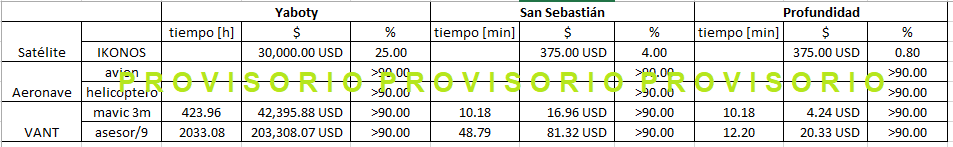
\includegraphics[width=\textwidth]{Imagenes/Tabla comparativa borrador.png}
     \hfill
     \caption{Tabla borrador}
        \label{Tabla_borrador}
\end{figure}
Obtener los datos y características técnicas de los sensores no es tarea sencilla. La información que suele figurar en los sitios web de los fabricantes o en los manuales, no suele ser la que se necesita para calcular. Por ejemplo la distancia focal no suele ser un dato que aparezca en la lista de especificaciones. Puede obtenerse de los metadatos asociados a una imagen que ha sido capturada con ese sensor.
Del mismo modo tampoco resulta sencillo obtener información sobre las tarifas de vuelos de relevamiento aéreo, ya sea tripulado o no. La información disponible es vaga y escueta, por ejemplo la hora de vuelo tripulado es de 240 dólares estadounidenses si se toma como base el dólar oficial (cotizado en 55 mil pesos argentinos, mayo 2023), y la de VANT es de 195 dólares estadounidenses (cotizado en 45 mil pesos argentinos, mayo 2023).
\subsubsection{Hardware}
Los que se pueden seleccionar con mayor grado de libertad son los que están relacionados con el hardware asociado a la tarea, como es el sensor de la cámara, o las características de funcionamiento de la aeronave no tripulada. Una cámara con mayor resolución demandará mayor espacio de almacenamiento. Asimismo si se trata de sensores ópticos en el rango del espectro visible, la posibilidad de operar se limitará a las horas diurnas. No así si se trata de sensores que trabajan en otro rango de longitudes de onda, como los infrarrojos, o sensores activos, como LiDAR.
\subsubsection{Marco regulatorio}

\subsubsection{Almacenamiento necesario}
Dependiendo de la resolución espacial y espectral de las imágenes, los requerimientos de almacenamiento aumentarán en proporción a las mismas. Siguiendo con el ejemplo antes expuesto, las casi seis millones y medio de fotografías en RGB, con 5 Megapíxeles por cada una, con una profundidad de color de 8 bit por canal necesitarían un espacio de almacenamiento de alrededor de 7,5 Terabytes.
\subsubsection{Cálculo presupuestario}
Partiendo de las características del terreno a relevar (su extensión) y de la plataforma usada para la captura (dron con cámara/sensor) es posible acotar un marco presupuestario para llevar a cabo la tarea. Con los datos recabados puede afirmarse que para un relevamiento aéreo de un área pequeña de veinte hectáreas, es conveniente un VANT, ya que el costo total no excedería los 10 dólares, mientras que en un avión tripulado el costo total sería por lo menos diez veces, y una imagen satelital tendría un costo de 375 dólares. En el caso de un área un poco más grande, de cien hectáreas, el costo total con VANT sigue siendo más bajo que con las otras plataformas, con menos de 50 dólares. Finalmente para el caso de un área mucho más grande, de varios miles de hectáreas como la reserva Yaboty, se torna más conveniente el avión tripulado con alrededor de 20 mil dólares estadounidenses, un poco más que la mitad de lo que cuesta la imagen satelital, y muy por debajo del costo del VANT, que supera holgadamente el millón de dólares.
%%%%%%%%%%%%%%%%%%%%%%%%%%%%%%%%%%%%%%%%% TABLA %%%%%%%%%%%%%%%%%%%%%%%%%%%%%%%%%%%%%%%%%%%%%%%%%%%%%%%%%
% Please add the following required packages to your document preamble:
% \usepackage{multirow}
% \usepackage[table,xcdraw]{xcolor}
% If you use beamer only pass "xcolor=table" option, i.e. \documentclass[xcolor=table]{beamer}
% \usepackage[normalem]{ulem}
% \useunder{\uline}{\ul}{}
% Please add the following required packages to your document preamble:
% \usepackage{multirow}
% \usepackage[table,xcdraw]{xcolor}
% If you use beamer only pass "xcolor=table" option, i.e. \documentclass[xcolor=table]{beamer}
% \usepackage[normalem]{ulem}
% \useunder{\uline}{\ul}{}
% Please add the following required packages to your document preamble:
% \usepackage{multirow}
% \usepackage[table,xcdraw]{xcolor}
% If you use beamer only pass "xcolor=table" option, i.e. \documentclass[xcolor=table]{beamer}
% \usepackage[normalem]{ulem}
% \useunder{\uline}{\ul}{}
% Please add the following required packages to your document preamble:
% \usepackage{multirow}
% \usepackage[table,xcdraw]{xcolor}
% If you use beamer only pass "xcolor=table" option, i.e. \documentclass[xcolor=table]{beamer}
% \usepackage[normalem]{ulem}
% \useunder{\uline}{\ul}{}
% Please add the following required packages to your document preamble:
% \usepackage{booktabs}
% \usepackage{graphicx}
% Please add the following required packages to your document preamble:
% \usepackage{booktabs}
% \usepackage{graphicx}
% Please add the following required packages to your document preamble:
% \usepackage{booktabs}
% \usepackage{multirow}
% \usepackage{graphicx}
% Please add the following required packages to your document preamble:
% \usepackage{multirow}
% \usepackage{graphicx}
% Please add the following required packages to your document preamble:
% \usepackage{multirow}
% \usepackage{graphicx}
% \usepackage[table,xcdraw]{xcolor}
% If you use beamer only pass "xcolor=table" option, i.e. \documentclass[xcolor=table]{beamer}
\begin{landscape}
\begin{table}[]

    \caption{Comparación de los tiempos y costos para cada plataforma}
    \label{tab:tabla}
   
    \begin{tabular}{cc|ccc|ccc|ccc|c|}
    \cline{3-12}
    \multicolumn{2}{c|}{} &
      \multicolumn{3}{c|}{\cellcolor[HTML]{68CBD0}\textbf{Yaboty}} &
      \multicolumn{3}{c|}{\cellcolor[HTML]{68CBD0}\textbf{San   Sebastián}} &
      \multicolumn{3}{c|}{\cellcolor[HTML]{68CBD0}\textbf{Profundidad}} &
       \\ \cline{3-11}
    \multicolumn{2}{c|}{\multirow{-2}{*}{}} &
      \multicolumn{1}{c|}{\cellcolor[HTML]{68CBD0}\textit{Tiempo {[}h{]}}} &
      \multicolumn{1}{c|}{\cellcolor[HTML]{68CBD0}\textit{\$}} &
      \cellcolor[HTML]{68CBD0}\textit{\%} &
      \multicolumn{1}{c|}{\cellcolor[HTML]{68CBD0}\textit{Tiempo {[}min{]}}} &
      \multicolumn{1}{c|}{\cellcolor[HTML]{68CBD0}\textit{\$}} &
      \cellcolor[HTML]{68CBD0}\textit{\%} &
      \multicolumn{1}{c|}{\cellcolor[HTML]{68CBD0}\textit{Tiempo {[}min{]}}} &
      \multicolumn{1}{c|}{\cellcolor[HTML]{68CBD0}\textit{\$}} &
      \cellcolor[HTML]{68CBD0}\textit{\%} &
      \multirow{-2}{*}{\textbf{Resolución espacial {[}cm/pixel{]}}} \\ \hline
    \multicolumn{1}{|c|}{\cellcolor[HTML]{9698ED}} &
      \cellcolor[HTML]{9698ED}Pleiades &
      \multicolumn{1}{c|}{} &
      \multicolumn{1}{c|}{37,500.00 USD} &
       &
      \multicolumn{1}{c|}{} &
      \multicolumn{1}{c|}{375.00 USD} &
       &
      \multicolumn{1}{c|}{} &
      \multicolumn{1}{c|}{375.00 USD} &
       &
       \\ \cline{2-12} 
    \multicolumn{1}{|c|}{\cellcolor[HTML]{9698ED}} &
      \cellcolor[HTML]{9698ED}Satellogic &
      \multicolumn{1}{c|}{} &
      \multicolumn{1}{c|}{37,500.00 USD} &
       &
      \multicolumn{1}{c|}{} &
      \multicolumn{1}{c|}{375.00 USD} &
       &
      \multicolumn{1}{c|}{} &
      \multicolumn{1}{c|}{375.00 USD} &
       &
       \\ \cline{2-12} 
    \multicolumn{1}{|c|}{\multirow{-3}{*}{\cellcolor[HTML]{9698ED}\textbf{Satélite}}} &
      \cellcolor[HTML]{9698ED}IKONOS &
      \multicolumn{1}{c|}{} &
      \multicolumn{1}{c|}{37,500.00 USD} &
      ? &
      \multicolumn{1}{c|}{} &
      \multicolumn{1}{c|}{375.00 USD} &
      4.00 &
      \multicolumn{1}{c|}{} &
      \multicolumn{1}{c|}{375.00 USD} &
      0.80 &
      96.35 \\ \hline
    \multicolumn{1}{|c|}{\cellcolor[HTML]{9698ED}} &
      \cellcolor[HTML]{9698ED}Ala fija &
      \multicolumn{1}{c|}{69.13} &
      \multicolumn{1}{c|}{6,912.77 USD} &
      \textgreater{}90.00 &
      \multicolumn{1}{c|}{2.24} &
      \multicolumn{1}{c|}{3.74 USD} &
      \textgreater{}90.00 &
      \multicolumn{1}{c|}{0.42} &
      \multicolumn{1}{c|}{0.70 USD} &
      \textgreater{}90.00 &
      10.21 \\ \cline{2-12} 
    \multicolumn{1}{|c|}{\multirow{-2}{*}{\cellcolor[HTML]{9698ED}\textbf{Aeronave}}} &
      \cellcolor[HTML]{9698ED}Ala rotativa &
      \multicolumn{1}{c|}{} &
      \multicolumn{1}{c|}{} &
      \textgreater{}90.00 &
      \multicolumn{1}{c|}{} &
      \multicolumn{1}{c|}{} &
      \textgreater{}90.00 &
      \multicolumn{1}{c|}{} &
      \multicolumn{1}{c|}{} &
      \textgreater{}90.00 &
       \\ \hline
    \multicolumn{1}{|c|}{\cellcolor[HTML]{9698ED}} &
      \cellcolor[HTML]{9698ED}mavic 3m &
      \multicolumn{1}{c|}{8645.64} &
      \multicolumn{1}{c|}{ 1,685,899.92  USD} &
      \textgreater{}90.00 &
      \multicolumn{1}{c|}{5.12} &
      \multicolumn{1}{c|}{8.53 USD} &
      \textgreater{}90.00 &
      \multicolumn{1}{c|}{1.22} &
      \multicolumn{1}{c|}{2.04 USD} &
      \textgreater{}90.00 &
      10.23 \\ \cline{2-12} 
    \multicolumn{1}{|c|}{\cellcolor[HTML]{9698ED}} &
      \cellcolor[HTML]{9698ED}asesor/9 &
      \multicolumn{1}{c|}{21666.57} &
      \multicolumn{1}{c|}{ 4,224,981.67 USD } &
      \textgreater{}90.00 &
      \multicolumn{1}{c|}{10.38} &
      \multicolumn{1}{c|}{17.30 USD} &
      \textgreater{}90.00 &
      \multicolumn{1}{c|}{2.19} &
      \multicolumn{1}{c|}{3.66 USD} &
      \textgreater{}90.00 &
      5.34 \\ \cline{2-12} 
    \multicolumn{1}{|c|}{\multirow{-3}{*}{\cellcolor[HTML]{9698ED}\textbf{VANT}}} &
      \cellcolor[HTML]{9698ED}mini 2 &
      \multicolumn{1}{c|}{18854.06} &
      \multicolumn{1}{c|}{ 3,676,541.38 USD } &
      \textgreater{}90.01 &
      \multicolumn{1}{c|}{9.34} &
      \multicolumn{1}{c|}{15.57 USD} &
      \textgreater{}90.01 &
      \multicolumn{1}{c|}{2.25} &
      \multicolumn{1}{c|}{3.75 USD} &
      \textgreater{}90.01 &
      3.47 \\ \hline
    \end{tabular}%

\end{table}
\end{landscape}
%%%%%%%%%%%%%%%%%%%%%%%%%%%%%%%%%%%%%%%%%%%%%%%%%%%%%%%%%%%%%%%%%%%%%%%%%%%%%%%%%%%%%%%%%%%%%%%%%%%%%%%%%


\section{Procesamiento de imágenes (Bloque 2)}

\subsection{Filtrado homomórfico (CRICTE 2017)}
\subsubsection{C1-Lógica difusa y procesamiento homomórfico (sombras)}
Según el modelo Stockham \cite{stockham_image_1972} una imagen puede descomponerse en dos partes, una la denominada iluminación y la otra componente es la reflexión. Llevadas al plano de frecuencias, se confirma el hecho de que la componente de iluminación tiene una variación más lenta, es decir, se corresponde con las frecuencias bajas. De modo similar, la componente de reflexión se corresponde con frecuencias altas \cite{oppenheim_nonlinear_1968}. Entendiendo esto, es factible implementar un filtrado en la imagen para realzar las sombras, separando la componente de iluminación de la de reflexión. Esta técnica fue utilizada en la remoción de sombras en imágenes de piezas de manufactura \cite{yang_research_2012} y en la detección automática de sombras en objetos oscuros \cite{etemadnia_automatic_2003}. En el presente trabajo, la aplicación a la detección de especies arbóreas es novedosa. 
Tomando como base el modelo de iluminación de Stockham para descomponer partes iluminadas de sombreadas, adoptando el concepto de frecuencia espacial, se implementó un procedimiento que incluía una etapa de filtrado homomórfico seguida de una etapa de aplicación de lógica difusa para discriminar sombras en imágenes aéreas de porciones de selva.
La imagen se modela como el producto de una componente de iluminación y otra de reflexión, que depende de las características del objeto iluminado. 
La ecuación que representa al filtro es
%%%%%%%%%%%%%%%%%%%%%%%%%%%%%%%%%%%%%% ECUACIÓN %%%%%%%%%%%%%%%%%%%%%%%%%%%%%%%%%%%%%%%%%%%%%%%%%%%%%%%%%
\\
\begin{equation}
	H(u,v)=1-((\gamma_H-\gamma_L)(1-e^{\frac{-cD^L(u,v)}{D^L_0}}+\gamma_L),\label{filtro homomorfico}
\end{equation}
\\
%%%%%%%%%%%%%%%%%%%%%%%%%%%%%%%%%%%%%%%%%%%%%%%%%%%%%%%%%%%%%%%%%%%%%%%%%%%%%%%%%%%%%%%%%%%%%%%%%%%%%%%%%  


donde $D_0$ es la frecuencia de corte, $c$ controla la forma y pendiente del filtro en la región de trancisión entre $\gamma_L$ y $\gamma_H$. $D(u,v)$ es la distancia al origen del plano de frecuencias.

Las imágenes a ser analizadas fueron obtenidas desde el sitio web Bing (poner en referencia de la dirección web del maps). Se seleccionaron imágenes de diferentes sitios de la Provincia de Misiones, correspondientes a selvas en parques y reservas, en los que se supone mayor presencia de especies de árboles de interés para el presente trabajo. 
En un primer paso se realizó la conversión de la imagen de color rojo, verde y azul (RGB) a la representación matiz, saturación e intensidad (HSI), trabajando sobre la componente de intensidad. En un paso siguiente se aplicó el logaritmo a la componente de intensidad de la imagen y seguidamente se obtuvo la transformada de Fourier de la misma, para poder procesar con el filtro de sombras. Se multiplicó la matriz de la imagen por la matriz que representa al filtro y, luego, al resultado se aplicó la transformada inversa de Fourier, la función inversa de logaritmo y la remoción de fase, tomando el módulo del número complejo, todo en orden sucesivo. Posteriormente se binarizó la imagen filtrada mediante un criterio de umbral de 0,75 en una escala en la que el valor 1 es blanco y 0 es negro. La imagen de salida del filtro de sombras presenta a las sombras resaltadas con píxeles de intensidad blancos. 
Luego se efectuó la selección de las sombras binarizadas, con lo que se descartaron las sombras que no revisten interés para el posterior conteo, estableciendo una ventana de enmascaramiento, que a los efectos prácticos es cuadrada y el criterio de clasificación es de 45\% de píxeles blancos. Una vez completas la binarización y la selección de sombras de interés, se realizó el conteo de las mismas. El diagrama de flujo de la fig. 3 describe las etapas del proceso completo. A los efectos de demostrar el grado de certeza del algoritmo, se comparó con la detección manual, variando el tamaño de la ventana de enmascaramiento. Se comprobó que eligiendo un tamaño de ventana de enmascaramiento igual a 20 por 20 píxeles se obtenía un acercamiento al criterio de selección manual.
En el proceso de binarización, se definió como umbral que correspondía a un valor de intensidad por encima del cual se trataba de sombras. En este caso el valor de intensidad fue de 0,75 en valores de intensidad de píxeles normalizados.
Para la selección de sombras binarizadas se recorrió la matriz de la imagen con una ventana de inspección que abarcaba 25 píxeles por lado, de modo que se evalúa un conjunto de 625 píxeles. Se estableció un umbral de 0,45 para clasificar las sombras, de modo que los recintos de píxeles blancos que superaban ese umbral eran catalogados como sombras de árboles grandes.
A los efectos de mostrar el funcionamiento del método de búsqueda y conteo de sombras, se exponen las fig. 4, 5 y 6 en las que se visualizan la imagen satelital en escala de grises de una porción de la reserva privada Sombra de Toro, ubicada en el norte de la provincia de Misiones, la imagen binarizada luego del filtrado homomórfico y las sombras seleccionadas, respectivamente.


\color{black} 
\subsection{Procesamiento morfológico (Pasantía)}
Partiendo de una imagen en escala de grises, se realizó una secuencia de pasos en los que se implementan diferentes filtros para identificar cada una
de las copas, de un modo que finalmente se obtuvo una imagen binarizada con la cual se pudo obtener un conteo de las copas. El primer paso consistió en hacer una clara identificación de los bordes y del área de
copas. Luego se aplicó un algoritmo de Rolling Ball \cite{sternberg_biomedical_1983} que produce un suavizado en los niveles de grises dentro de las copas. En una siguiente etapa, distinguiendo copas
grandes de pequeñas, se identificaban huecos en las copas grandes, para posteriormente rellenarlos con un valor promedio. Una vez rellenos todos los huecos y uniformadas todas las copas, se procede a segmentarlas, obteniéndose una imagen binarizada, con cada copa de árbol aislada e identificada en su posición.

Secuencia de actividades para el tratamiento de las imágenes\\
1. Preprocesamiento\\
2. Eliminación de áreas sin sombra\\
3. Primera identificación de objetos oscuros\\
4. Relleno de sombras en copas\\
5. Identificación y relleno de huecos en grandes copas\\
6. Segunda identificación de objetos oscuros\\
7. Búsqueda de pequeños huecos en grandes copas\\
8. Homogeneización de escala de grises en grandes árboles\\
9. Extracción de copas de segmentación\\
10.  Delineación de copas individuales\\


3 Evaluación de la influencia de diferentes parámetros en los algoritmos Se evaluó el desempeño de los algoritmos modificando en un determinado rango el
valor de distintos parámetros en cada etapa del procesamiento, para observar en qué modo se ven afectados los resultados. Se procedió a lo que se denomina “Gridsearch”, estableciendo valores de parámetros en grillas y los correspondientes resultados del procesamiento de las imágenes. En este procedimiento se evidencia la importancia y la vinculación que tienen los parámetros en las diferentes etapas con la resolución espacial de la imagen con la que se trabaja. En tanto en la última etapa se observó que el umbral
que se definió para separar (y por lo tanto binarizar la imagen) las copas segmentadas, en el artículo de referencia sugiere utilizar el umbral del 0,001 percentil, pero al hacer la prueba de Gridsearch con diferentes valores hasta el 0,9 percentil, resultaba notable que excepto el correspondiente al percentil 0,9 los demás resultados no eran visiblemente diferentes.



\color{cyan} %color de texto con 70-80 % o más de avance
\subsection{Invariante de color (paper RSASE)}
\subsubsection{Metodología propuesta IIC}
En esta sección se describen los pasos del método de procesamiento necesarios para obtener la máscara automática de sombras de la imagen aérea. La figura \ref{diagrama_procesamiento} representa la secuencia de procesamiento.

\begin{figure}
    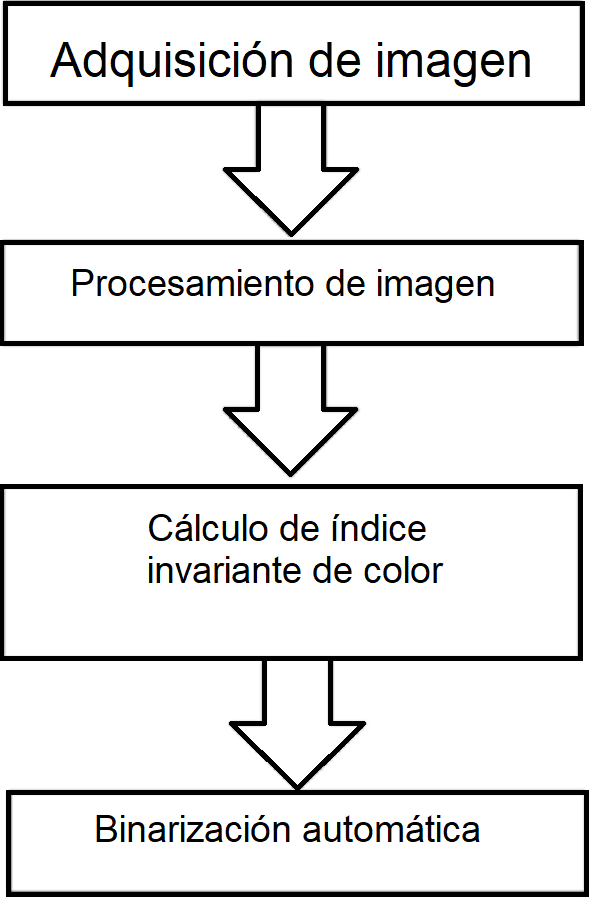
\includegraphics[width=\textwidth]{Imagenes/flowchart.png}
     \hfill
     \caption{Diagrama del procesamiento}
    \label{diagrama_procesamiento}
\end{figure}

\paragraph{Adquisición de la imagen}
El punto de partida de la metodología propuesta es la captura de imágenes aéreas. Entre los pocos requerimientos en esta etapa se destaca que las condiciones de luz solar deben ser las apropiadas para generar proyecciones de sombra. Aquí se consideran imagenes representativas de un área de selva nativa en la provincia de Misiones, Argentina, que han sido capturadas mediante VANT sobrevolando porciones de selva en parques y reservas naturales, en las cuales habría presencia de ejemplares de árboles de interés. Para garantizar una mejor captura de imágenes con sombra, se seleccionó un intervalo de tiempo que abarca desde las 3 p.m. hasta las 4 p.m., que es cuando la posición relativa del sol facilita la proyección de sombras sobre el dosel. Las imágenes fueron capturadas durante el invierno meridional, específicamente en el mes de agosto, cuando las sombras proyectadas son mayores para ese horario. Se usó un VANT modelo Mini 2 del fabricante DJI, equipado con una cámara con resolución de 12 Megapíxeles. La altura de vuelo sobre el terreno fue de 50 metros, y el modo en que estuvo configurada la cámara era automático. Las imágens capturadas están en formato JPG con una resolución de 4000 x 2250 píxeles, con una resolución espacial de 3 cm/pixel aproximadamente. Para ejecutar el algoritmo se usó una computadora laptop común con un procesador Intel Core i5. En cuanto a los scripts, están basados en códigos de Octave. Se analizó un total de 19 imágenes.

\paragraph{Preprocesamiento de imagen} \label{Metodología}
Para facilitar el procesamiento y posterior análisis, las imágenes de los diferentes sitios deben ser recortadas par anormalizar el tamaó y ser filtradas para estandarizar algunos atributos.
\paragraph{Cálculo de índice invariante de color}
Con base en imágenes filtradas RGB, el invariante de color $\Psi$ se calcula por medio de la ecuación \ref{invariante de color}
 %%%%%%%%%%%%%%%%%%%%%%%%%%%%%%%%%%%%%% ECUACIÓN %%%%%%%%%%%%%%%%%%%%%%%%%%%%%%%%%%%%%%%%%%%%%%%%%%%%%%%%%
\\
\begin{equation}
	\Psi=\frac{4}{\pi} arctan\left(\frac{B\textsubscript{1}-B\textsubscript{2}}{B\textsubscript{1}+B\textsubscript{2}}\right),\label{invariante de color}
\end{equation}
\\
%%%%%%%%%%%%%%%%%%%%%%%%%%%%%%%%%%%%%%%%%%%%%%%%%%%%%%%%%%%%%%%%%%%%%%%%%%%%%%%%%%%%%%%%%%%%%%%%%%%%%%%%%
 donde $B_1$ y $B_2$ son dos bandas diferentes de color, rojo, verde o azul. El índice invariante de color $\Psi$ toma un valor entre -1 y 1. Si se aplica la ecuación a las bandas correspondientes $B_1$ y $B_2$, el resultado es una matriz de idéntico tamaño al de la imagen, en la que cada píxel contiene el valor del índice invariante de color. Según sea la combinación entre bandas, hay hasta seis posibilidades, siendo una mitad complementaria de la otra mitad. Por esta razón sólo se tienen en cuenta tres de esas posibilidades. La matriz de índice invariante de color se usó para analizar las partes sombreadas y no sombreadas de la imagen. Así, para las tres combinaciones a implementar, se describen en las ecuaciones \ref{psibr}, \ref{psibg} y \ref{psigr}:
 \\
 \\
\begin{equation}
	\Psi_{BR}=\frac{4}{\pi} arctan\left(\frac{B\textsubscript{B}-B\textsubscript{R}}{B\textsubscript{B}+B\textsubscript{R}}\right),\label{psibr}
\end{equation}
\\
\\
\begin{equation}
	\Psi_{BG}=\frac{4}{\pi} arctan\left(\frac{B\textsubscript{B}-B\textsubscript{G}}{B\textsubscript{B}+B\textsubscript{G}}\right),\label{psibg}
\end{equation}
\\
\\
\begin{equation}
	\Psi_{GR}=\frac{4}{\pi} arctan\left(\frac{B\textsubscript{G}-B\textsubscript{R}}{B\textsubscript{G}+B\textsubscript{R}}\right),\label{psigr}
\end{equation}
\\
donde $B_{B}$, $B_{G}$, y $B_{R}$ son los canales azul, verde y rojo respectivamente.
\paragraph{Binarización automática}
 La binarización permite separar la imagen en dos regiones, con sombra y sin sombra, mediante la matriz de índice invariante de color y un valor de umbral, calculado como la frecuencia acumulada de la distribución de valores individuales de IIC. Esta máscara que se obtiene, denominada máscara automática, se compone de píxeles de valores 1 y 0, correspondiendo el valor de 1 al de las regiones sombreadas de la imagen. En la composición de la máscara binaria se asume un valor de 1 (visualizado en blanco) para las regiones sombreadas. Tomando la distribución de frecuencia acumulada del índice invariante de color, se determina el valor umbral que excede los percentiles 60º, 70º, 80º, 85º, 90º y 95º. De este modo, en el presente trabajo, se obtienen seis máscaras, cada una correspondiente al valor de umbral de cada percentil. Luego el valor de umbral es variable y es calculado para cada imagen para un percentil determinado. La calidad de cada máscara automática obtenida es evaluada al compararse con una máscara manual obtenida por un experto humano para la correspondiente imagen.

\paragraph{Comparación cuantitativa con un índice de calidad}
Para establecer un índice de calidad (QI) del desempeño de la selección automática, se proponen tres índices: el primero ($QI_1$) se obtiene del cociente entre la suma de todos los píxeles de la matriz binaria, obtenida como consecuencia de la intersección de la máscara manual y la máscara automática, y la suma de todos los elementos de la máscara manual (\ref{qi1}). El segundo índice ($QI_2$) se obtiene dividiendo la suma de elementos de la intersección por la suma de los elementos de la máscara automática (\ref{qi2}); y el tercer índice ($QI_3$) se obtiene dividiendo la suma de los elementos de la intersección por la suma de los elementos de la unión de la máscara manual y automática (\ref{qi3}.
\\
\\
 \begin{equation}
    QI_1=\frac{\Sigma _{i,j}(M_M\cap M_A )}{\Sigma _{i,j}(M_M ) }
    \label{qi1}
\end{equation}
\\
\\
 \begin{equation}
    QI_2=\frac{\Sigma _{i,j}(M_M\cap M_A )}{\Sigma _{i,j}(M_A ) }
    \label{qi2}
\end{equation}
\\
\\
\begin{equation}
    QI_3=\frac{\Sigma _{i,j}(M_M\cap M_A )}{\Sigma _{i,j}(M_M \cup M_A ) }
    \label{qi3}
\end{equation}
\\
\\
Donde $M_M$ es la máscara binaria manual y $M_A$ es la máscara binaria automática. Cada uno de los índices precedentes toma valores de 0 a 1, siendo 0 el caso en que no hay ninguna coincidencia entre máscaras, y 1 indica plena coincidencia. Para los tres índices, el numerador es la intersección entre ambas máscaras, manual y automática, ya que es un buen indicador de coincidencia entre ambas. El denominador en tanto da un valor de referencia que parametriza el índice. La intersección y la unión son operaciones lógicas que se aplican a cada píxel, de modo que es una condición necesaria que sendas máscaras binarias automática y manual que serán comparadas entre sí, sean del mismo tamaño y de áreas de captura coincidentes. En un nivel de píxel, la intersección es una operación lógica "and", por lo que, al ser cero uno de sendos píxeles comparados, el resultado de la operación dará cero. Por otro lado, la unión implica una operación a nivel de píxel de tipo "or", y siendo uno de sendos píxeles de valor uno, el resultado será uno. El objetivo de este índice es evaluar cuanto se asemeja la selección automática del algoritmo a la selección manual. Así, el mayor valor que corresponde a 1 implica una selección automática exacta, mientras que valores más bajos cercanos a cero corresponden a una pobre correlación entre sendas selecciones.


\paragraph{Etapa de filtrado}
Para quitar el ruido de la imagen, se implementa un filtro de mediana. Para evaluar cómo la etapa de filtrado afecta el desempeño de la selección automática, se realizaron para cada imagen tres pruebas con diferentes configuraciones de filtro, con vecindad de tres por tres, seis por seis, y  doce por doce pixeles. Para cada caso se propuso un conjunto de tres índices de calidad, descriptos en las ecuaciones \ref{qi5}, \ref{qi6} y \ref{qi7}
\\
\\
 \begin{equation}
    QI_5=\frac{\Sigma _{i,j}(M_{NF}\cap M_{WF})}{\Sigma _{i,j}(M_{NF}) }
    \label{qi5}
\end{equation}
\\
\\
 \begin{equation}
    QI_6=\frac{\Sigma_{i,j}(M_{NF}\cap M_{WF})}{\Sigma _{i,j}(M_{WF}) }
    \label{qi6}
\end{equation}
\\
\\
\begin{equation}
    QI_7=\frac{\Sigma _{i,j}(M_{NF}\cap M_{WF})}{\Sigma _{i,j}(M_{NF}\cup M_{WF}) }
    \label{qi7}
\end{equation}
\\
\\
en donde $M_{NF}$ es la máscara binaria automática obtenida sin filtrado, y $M_{WF}$ es la obtenida luego de la etapa de filtrado.

\subsubsection{Validación IIC} \label{Validacion}
Superponiendo a una imagen las dos máscaras, una obtenida en forma manual y otra en forma automática, tres expertos realizaron un análisis, calificando el grado de ajuste entre ambas máscaras como "bueno", "regular" o "malo". Este procedimiento fue aplicado a cada una de las 19 imágenes analizadas, de modo que se obtuvieron 19 máscaras automáticas por medio del algoritmo para ser comparadas con las respectivas máscaras obtenidas en forma manual. Las superposiciones calificadas como "buenas" o "regulares" son usadas para seleccionar la mejor máscara automática. Un procedimiento similar se siguió para evaluar el filtrado de la imagen.

\color{black} 
\subsection{Machine learning (¿?)}




%Las Tesis  en el marco de la Carrera del Doctorado en Ciencias Aplicadas (DCA) deberán ser escritas en idioma Español, utilizando letra tipo Arial, tamaño 11 puntos, y formato de hojas tipo A4, numeradas en el margen inferior derecho, con interlineado 1,5; sin separación automática de sílabas al fin de línea y con los cuatro márgenes de 2,5 cm.

%El contenido de las Tesis deberá incluir los siguientes ítems y en el siguiente orden:\newline
%●	Carátula (con el formato solicitado por el DCA que se adjunta al presente Anexo)\newline
%●	Agradecimientos\newline
%●	Índice\newline
%●	Listado de Abreviaturas (en caso de que lo considere conveniente)\newline
%●	Resumen en Español\newline
%●	Palabras Claves en Español (tres a seis palabras claves separadas por comas. La primera letra de cada palabra clave debe empezar con mayúscula)\newline
%●	Resumen en Inglés (Abstract)\newline
%●	Palabras Claves en Inglés (tres a seis palabras claves separadas por comas. La primera letra de cada palabra clave debe empezar con mayúscula)\newline
%●	Capítulo 1: Introducción (deberá contener el planteo del problema a resolver, los objetivos generales y específicos y una breve explicación de lo que versará la Tesis)\newline
%●	Capítulo 2: Marco Teórico\newline
%●	Capítulo 3: Metodología\newline
%●	Capítulo 4: Resultados y Discusión (O bien, se podrá presentar en dos Capítulos separados: Capítulo 4: Resultados y Capítulo 5: Discusión)\newline
%●	Capítulo 5: Conclusiones (Deben presentarse en párrafos cortos y concretos. No deben hacer referencia a trabajos futuros ni a hipótesis no incluidas en el trabajo).\newline
%●	Recomendaciones para Trabajos Futuros\newline
%●	Producción Científica (surgida del trabajo de Tesis)\newline
%✔	Publicaciones en Revistas y Capítulos de Libros\newline
%✔	Presentaciones a Congresos\newline
%●	Proyecto/s de Investigación dentro del/los cual/es se desarrolló la Tesis (si hubiera/n)\newline
%●	Beca/s y Subsidio/s con los que se financió la Tesis (si hubieran)\newline
%●	Apéndices o Anexos (se reservan para detallar técnicas originales utilizadas o análisis teóricos que impedirían seguir fluidamente el trabajo si se incluyeran en el texto). Las tablas y figuras de los apéndices o anexos deben comenzar otra numeración diferente a la de los capítulos.\newline

%Aclaraciones

%⮚	El listado de Referencias bibliográficas se podrá incorporar al final de cada capítulo, ó todas juntas al final de la Tesis, las mismas serán listadas en el orden en que aparecen citadas en el texto. \newline
%Formato de las Referencias\newline
%Estilo de las Referencias\newline
%En el texto de la Tesis: indique las referencias por número (s) entre corchetes en línea con el texto. Cuando se menciona a los autores, siempre se deben proporcionar los números de referencia.
%Ejemplo: '..... como se demostró [3,6]. Barnaby y Jones [8] obtuvieron un resultado diferente ... '
%Lista de Referencias\newline
%Numere las referencias (números entre corchetes) en la lista en el orden en que aparecen en el texto, como se indica a continuación:5
%\paragraph{Referencia a una publicación de revista}
%[1] J. van der Geer, J.A.J. Hanraads, R.A. Lupton, The art of writing a scientific article, J. Sci. Commun. 163 (2010) 51–59.https://doi.org/10.1016/j.Sc.2010.00372.
%\paragraph{Referencia a una publicación de revista con un número de artículo}
%[2] J. van der Geer, J.A.J. Hanraads, R.A. Lupton, 2018. The art of writing a scientific article.Heliyon. 19, e00205.https://doi.org/10.1016/j.heliyon.2018.e00205.
%\paragraph{Referencia a un libro}
%[3] W. Strunk Jr., E.B. White, The Elements of Style, fourth ed., Longman, New York, 2000.
%\paragraph{Referencia a un capítulo en un libro editado}
%[4] G.R. Mettam, L.B. Adams, How to prepare an electronic version of your article, in: B.S. Jones, R.Z. Smith (Eds.), Introduction to the Electronic Age, E-Publishing Inc., New York, 2009, pp. 281–304.
%\paragraph{Referencia a un sitio} web
%[5] Cancer Research UK, Cancer statistics reports for the UK. http://www.cancerresearchuk.org/ aboutcancer/statistics/cancerstatsreport/, 2003 (accessed 13 March 2003).
%\paragraph{Referencia a un conjunto de datos: [conjunto de datos]}
%[6] M. Oguro, S. Imahiro, S. Saito, T. Nakashizuka, Mortality data for Japanese oak wilt disease and surrounding forest compositions, Mendeley Data, v1, 2015. https://doi.org/10.17632/ xwj98nb39r.1
%⮚	Las figuras (gráficos, cuadros, fotografías, otros) deberán numerarse correlativamente en el orden de aparición en el texto y deberán incluir un breve título explicativo en la parte inferior de la figura. Las imágenes y fotografías se designarán como figuras.\newline
%%%%%%%%%%%%%%%%%%%%%%%%%%%%%%%%%%%%%%% FIGURA %%%%%%%%%%%%%%%%%%%%%%%%%%%%%%%%%%%%%%%%%%%%%%%%%%%%%%%%%
%\begin{figure}[ht!]
%    \centering
%    \captionsetup{justification=centering}
%    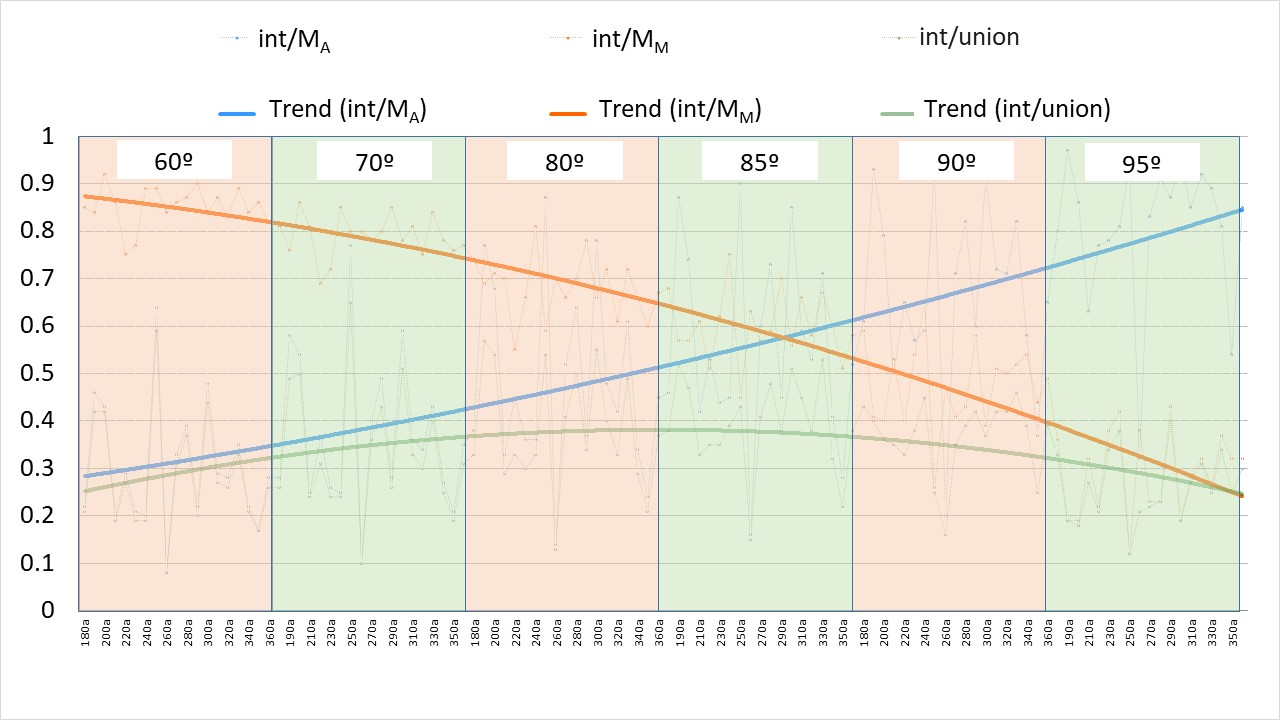
\includegraphics[width=8cm]{grafico.jpg}
%    \caption{Quality Index as a function of the percentile, for the different forest image used. QI\textsubscript{1} in orange, QI\textsubscript{2} in blue and QI\textsubscript{3} in green. The invariant color index used is ψ\textsubscript{BR}}	
 %   \label{qi}
%\end{figure}
%%%%%%%%%%%%%%%%%%%%%%%%%%%%%%%%%%%%%%%%%%%%%%%%%%%%%%%%%%%%%%%%%%%%%%%%%%%%%%%%%%%%%%%%%%%%%%%%%%%%%%%%%
%⮚	Las tablas deberán numerarse correlativamente según su orden de aparición en el texto y en forma independiente de las figuras. Deberán incluir un título explicativo en su parte superior. De ser necesario se agregarán al pie notas explicativas para detallar abreviaturas, signos, medidas, otros, de tal manera que el lector pueda comprender su contenido sin recurrir al texto.
%%%%%%%%%%%%%%%%%%%%%%%%%%%%%%%%%%%%%%%%% TABLA %%%%%%%%%%%%%%%%%%%%%%%%%%%%%%%%%%%%%%%%%%%%%%%%%%%%%%%%%
%\begin{table}[H]
  %  \centering
   % \caption{Evaluation of the superposition of both masks. the manual and the automatic. carried on by the group of experts}
    %\begin{tabular}{|c|c|c|c|c|c|c|c|}
     %  \hline
      %  COLOR INVARIANT INDEX & \multicolumn{6}{ |c|}{\textpsi \textsubscript{BR}}\\%\multicolumn{6}{ }{ |c|} \\
       % \hline
        %PERCENTILE & 60 & 70 & 80 & 85 & 90 & 95\\
        %\hline
        %GOOD & 0.0 & 0.0 & 4.5 & 15.8 & 20.5 & 0.0\\
        %\hline
        %REGULAR & 0.0 & 4.5 & 27.3 & 21.1 & 54.5 & 57.9\\
        %\hline
        %BAD & 100.0 & 95.5 & 68.2 & 63.2 & 25.0 & 42.1\\
        %\hline
        %COLOR INVARIANT INDEX & \multicolumn{6}{ |c|}{\textpsi \textsubscript{BG}}\\
        %\hline
        %PERCENTILE & 60 & 70 & 80 & 85 & 90 & 95\\
        %\hline
        %GOOD & 0.0 & 0.0 & 0.0 & 5.3 & 5.3 & 5.3\\
        %\hline
        %REGULAR & 0.0 & 5.3 & 10.5 & 15.8 & 42.1 & 21.1\\
        %\hline
        %BAD & 100.0 & 94.7 & 89.5 & 78.9 & 52.6 & 73.7\\
        %\hline
        %COLOR INVARIANT INDEX & \multicolumn{6}{|c|}{ \textpsi \textsubscript{GR}}\\
        %\hline
        %PERCENTILE & 60 & 70 & 80 & 85 & 90 & 95\\
        %\hline
        %GOOD & 0.0 & 0.0 & 0.0 & 0.0 & 0.0 & 0.0\\
        %\hline
        %REGULAR & 0.0 & 0.0 & 0.0 & 0.0 & 15.8 & 15.8\\
        %\hline
        %BAD & 100.0 & 100.0 & 100.0 & 100.0 & 84.2 & 84.2\\
        %\hline
    %\end{tabular}
    %\\
    %\raggedleft
    %\label{tablita}
%\end{table}
%%%%%%%%%%%%%%%%%%%%%%%%%%%%%%%%%%%%%%%%%%%%%%%%%%%%%%%%%%%%%%%%%%%%%%%%%%%%%%%%%%%%%%%%%%%%%%%%%%%%%%%%%
%⮚	Las fórmulas y expresiones matemáticas deberán ser escritas dejando dos espacios sobre, debajo y entre cada una de ellas.
%%%%%%%%%%%%%%%%%%%%%%%%%%%%%%%%%%%%%% ECUACIÓN %%%%%%%%%%%%%%%%%%%%%%%%%%%%%%%%%%%%%%%%%%%%%%%%%%%%%%%%%
%\begin{equation}
%	\psi=\frac{4}{\pi} arctan\left(\frac{B\textsubscript{1}-B\textsubscript{2}}{B\textsubscript{1}+B\textsubscript{2}}\right),\label{eq1}
%\end{equation}
%%%%%%%%%%%%%%%%%%%%%%%%%%%%%%%%%%%%%%%%%%%%%%%%%%%%%%%%%%%%%%%%%%%%%%%%%%%%%%%%%%%%%%%%%%%%%%%%%%%%%%%%%
%Las fórmulas se ajustarán al margen izquierdo y serán numeradas correlativamente y entre paréntesis sobre el margen derecho. Debe quedar definido el significado y las unidades utilizadas en cada término de las expresiones.

%⮚	Unidades: debe utilizarse el sistema internacional de unidades (SI).
